\newpage 

\subsection{Building Transistors: The Chemistry of Silicon}

\noindent
To even begin to manage currents and voltages, we will need a way to control the flow of electricity:

\begin{Def}[Transistor]

    \label{def:transistor}

  A \textbf{transistor} is a small electronic semiconductor device. A \textbf{semiconductor} (e.g., silicon) is a material with electrical 
    conductivity between that of a \textbf{conductor} (great electricity conductor) and an \textbf{insulator}
    (inhibits electric flow). Transistors fall into two broad families:

  \begin{itemize}
    \item \textbf{Bipolar Junction Transistor (BJT):} a current-controlled device with three terminals (pins),
    \begin{itemize}
        \item \textbf{Emitter (E):} current flows \emph{out}.
        \item \textbf{Base (B):} controls operation.
        \item \textbf{Collector (C):} current flows \emph{in}.
    \end{itemize}
    \item \textbf{Field-Effect Transistor (FET):} a voltage-controlled device with three terminals,
    \begin{itemize}
        \item \textbf{Source (S):} current flows \emph{in}.
        \item \textbf{Gate (G):} controls operation.
        \item \textbf{Drain (D):} current flows \emph{out}.
    \end{itemize}
  \end{itemize}

  \noindent
  Low-power transistors are molded in an epoxy (resin) package. Higher-power transistors often use a metal tab or ``can'' that you bolt to a \textbf{heat sink} (a metal object that dissipates heat).

  Pin order and package style vary by model; check the \textbf{part number} and manufacturer's \textbf{datasheet} for exact details \cite{what_is_transistor2022, engineermindset2024mosfet}.
\end{Def}

\begin{figure}[ht!]
  \centering
  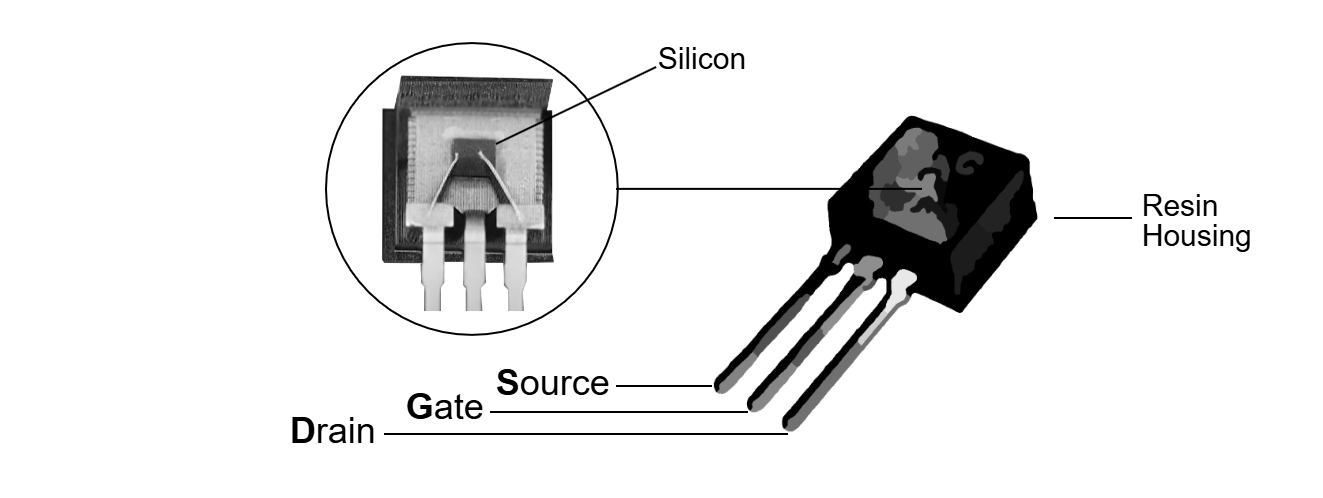
\includegraphics[width=\textwidth]{Sections/circuits/transistor.png}
  \caption{Cross-section of a discrete transistor: a silicon die (center) is bonded to three metal leads, all
    encased in an epoxy package.  A metal tab (not shown) may be added for heatsinking.}
  \label{fig:transistor}
\end{figure}

\newpage 



\begin{theo}[FETs over BJTs]

  \label{theo:why_mosfets_preferred}

  A BJT needs continuous base current, which wastes energy. A MOSFET only requires its gate to be charged or discharged (i.e., voltage applied or removed), which is more efficient.
\end{theo}

\noindent 
Now we briefly step into chemistry for completeness sake to understand differing silicon charges:
\begin{Def}[Anotomy of an Atom]

    \label{def:atom}

    An \textbf{atom} is the smallest unit of matter that retains the properties of an element. It consists of three main subatomic particles:
    \begin{itemize}
        \item \textbf{Protons:} Positively charged particles found in the nucleus.
        \item \textbf{Neutrons:} Neutral particles also found in the nucleus (same size as protons).
        \item \textbf{Electrons:} About the same charge as proton, but negative, and about 1800x smaller and lighter than a proton.
    \end{itemize}

    \noindent
    Protons and neutrons are tightly packed together in a space called the \textbf{nucleus}, gaining the name \textbf{nucleons};
    Electrons orbit the nucleus at discrete distances called \textbf{shells} or \textbf{energy levels}. 
    \underline{The number of protons in the nucleus defines the element (i.e., specifications).} E.g., 79 protons will 
    always be gold.

    Opposite charges attract, causing an \textbf{orbital space}, in which subatomic particles never collide (i.e., alike orbiting planets). Neutrons act as a buffer between protons (e.g., Silver is 
    stable with 60 or 62 neutrons, but unstable with 61). Atoms with different number of neutrons are called \textbf{isotopes}, latin for ``same place''.
    Electrons may jump between shells and atoms. If there is a greater number of electrons to protons, the atom is \textbf{negatively charged} (anions), otherwise it is \textbf{positively charged} (cations)
    \cite{crashcourse2013nucleus}.
\end{Def}

\begin{Def}[Periodic Table]

    \label{def:periodic_table}

    The \textbf{Periodic Table of Elements} organizes all known elements by the number of protons in their nuclei. This is called an \textbf{atomic number} (e.g., 
    gold's atomic number is 79). Elements are abbreviated from their latin translations (e.g., gold is \textbf{aurum}, AU, which means ``shining dawn'').
    There are 118 elements, with 80 being stable and the rest being unstable isotopes. Anything past 82 protons (lead) is 
    unstable, undergoing radioactive decay.
\end{Def}

\begin{Tip} The periodic table is complete, hence movies that claim ``we discovered a new element!'' truly deserve science-fiction as their defining genre.
\end{Tip}
\newpage 
\noindent
We'll stop with the chemistry dive after these next two critical definitions

\begin{Def}[Shell Capacities \& Valence Electrons]

    \label{def:valence_electrons}

    The first shell of any atom can hold up to 2 electrons, and the second 8. From 1-20 periodic elements, the third and fourth 
    shells can hold 8 and 2 respectively. A \emph{full} shell is considered \textbf{stable}, otherwise it is \textbf{unstable}.
    This arrangement of electrons within the shells is called the \textbf{electron configuration} (EC) of the atom.
    An EC is written as a n-tuple, starting with the inner-most shell (e.g., 2, 8, 8, 2 for calcium).

    
    The outer most shell is called the \textbf{valence shell}. An atom's \textbf{valency} (the number of electrons in the valence shell) determines whether a chemical reaction will occur.
     If an atom is stable (i.e., full valence shell), it will not react with other atoms.
    Unstable atoms \emph{strive} to become stable by either gaining, losing, or sharing electrons with other atoms \cite{infinitylearn2018concept}.
\end{Def}

\begin{Def}[Chemical Bonds -- Molecules \& Compounds]

    \label{def:chemical_bonds}

    The act of atoms joining together (e.g., sharing electrons, which is called a \textbf{covalent bond}), forms a \textbf{molecule}. 
    Concretely, a molecule is a merger of two or more elements. We use subscripts to denote the number of atoms in a molecule (e.g., H$_2$O is water, with two hydrogen atoms and one oxygen atom).
    \textbf{Compounds} are a subset class of molecules that consists only of two more more \textbf{different} elements (e.g., H$_2$O is a compound, but O$_2$ is not, as it only has one element, oxygen)  \cite{breslyn2013molecule}.
\end{Def}
\noindent
Now to what we've been waiting for:
\begin{Def}[Doping -- N-type \& P-type Silicon]

    \label{def:doping}

    Silicon has 14 atoms, with an EC of (2, 8, 4); Hence silicon is unstable. If we view silicon (Si) as a 3D lattice (a string of Si atoms in 3D grid),
    each Si atom will share its four valence electrons with it neighbors to become stable (covalent bonding). This creates a \textbf{silicon crystal}.\\

    \noindent
    Adding another element to the silicon lattice is called \textbf{doping}. We 
    are interested in two types of doping \cite{engineermindset2024mosfet}:
    \begin{itemize}
        \item \textbf{N-type:} When adding an element like phosphorus (P), EC of (2, 8, 5), is added to the silicon lattice, one electron goes unused after the covalent bonding. This free electron creates a \textbf{negative charge carrier} (hence N-type).
        \item \textbf{P-type:} Conversely, adding boron (B), EC of (2, 8, 3), creates a \textbf{positive charge carrier} (hence P-type). This is because boron won't have 
        enough to share with its neighbors, causing \textbf{holes} (absence of electrons), overall lowering the density of electrons.
    \end{itemize}
\end{Def}

\newpage 

\noindent 
Let's visualize what we've learned so far:

\begin{figure}[ht!]

  \centering
  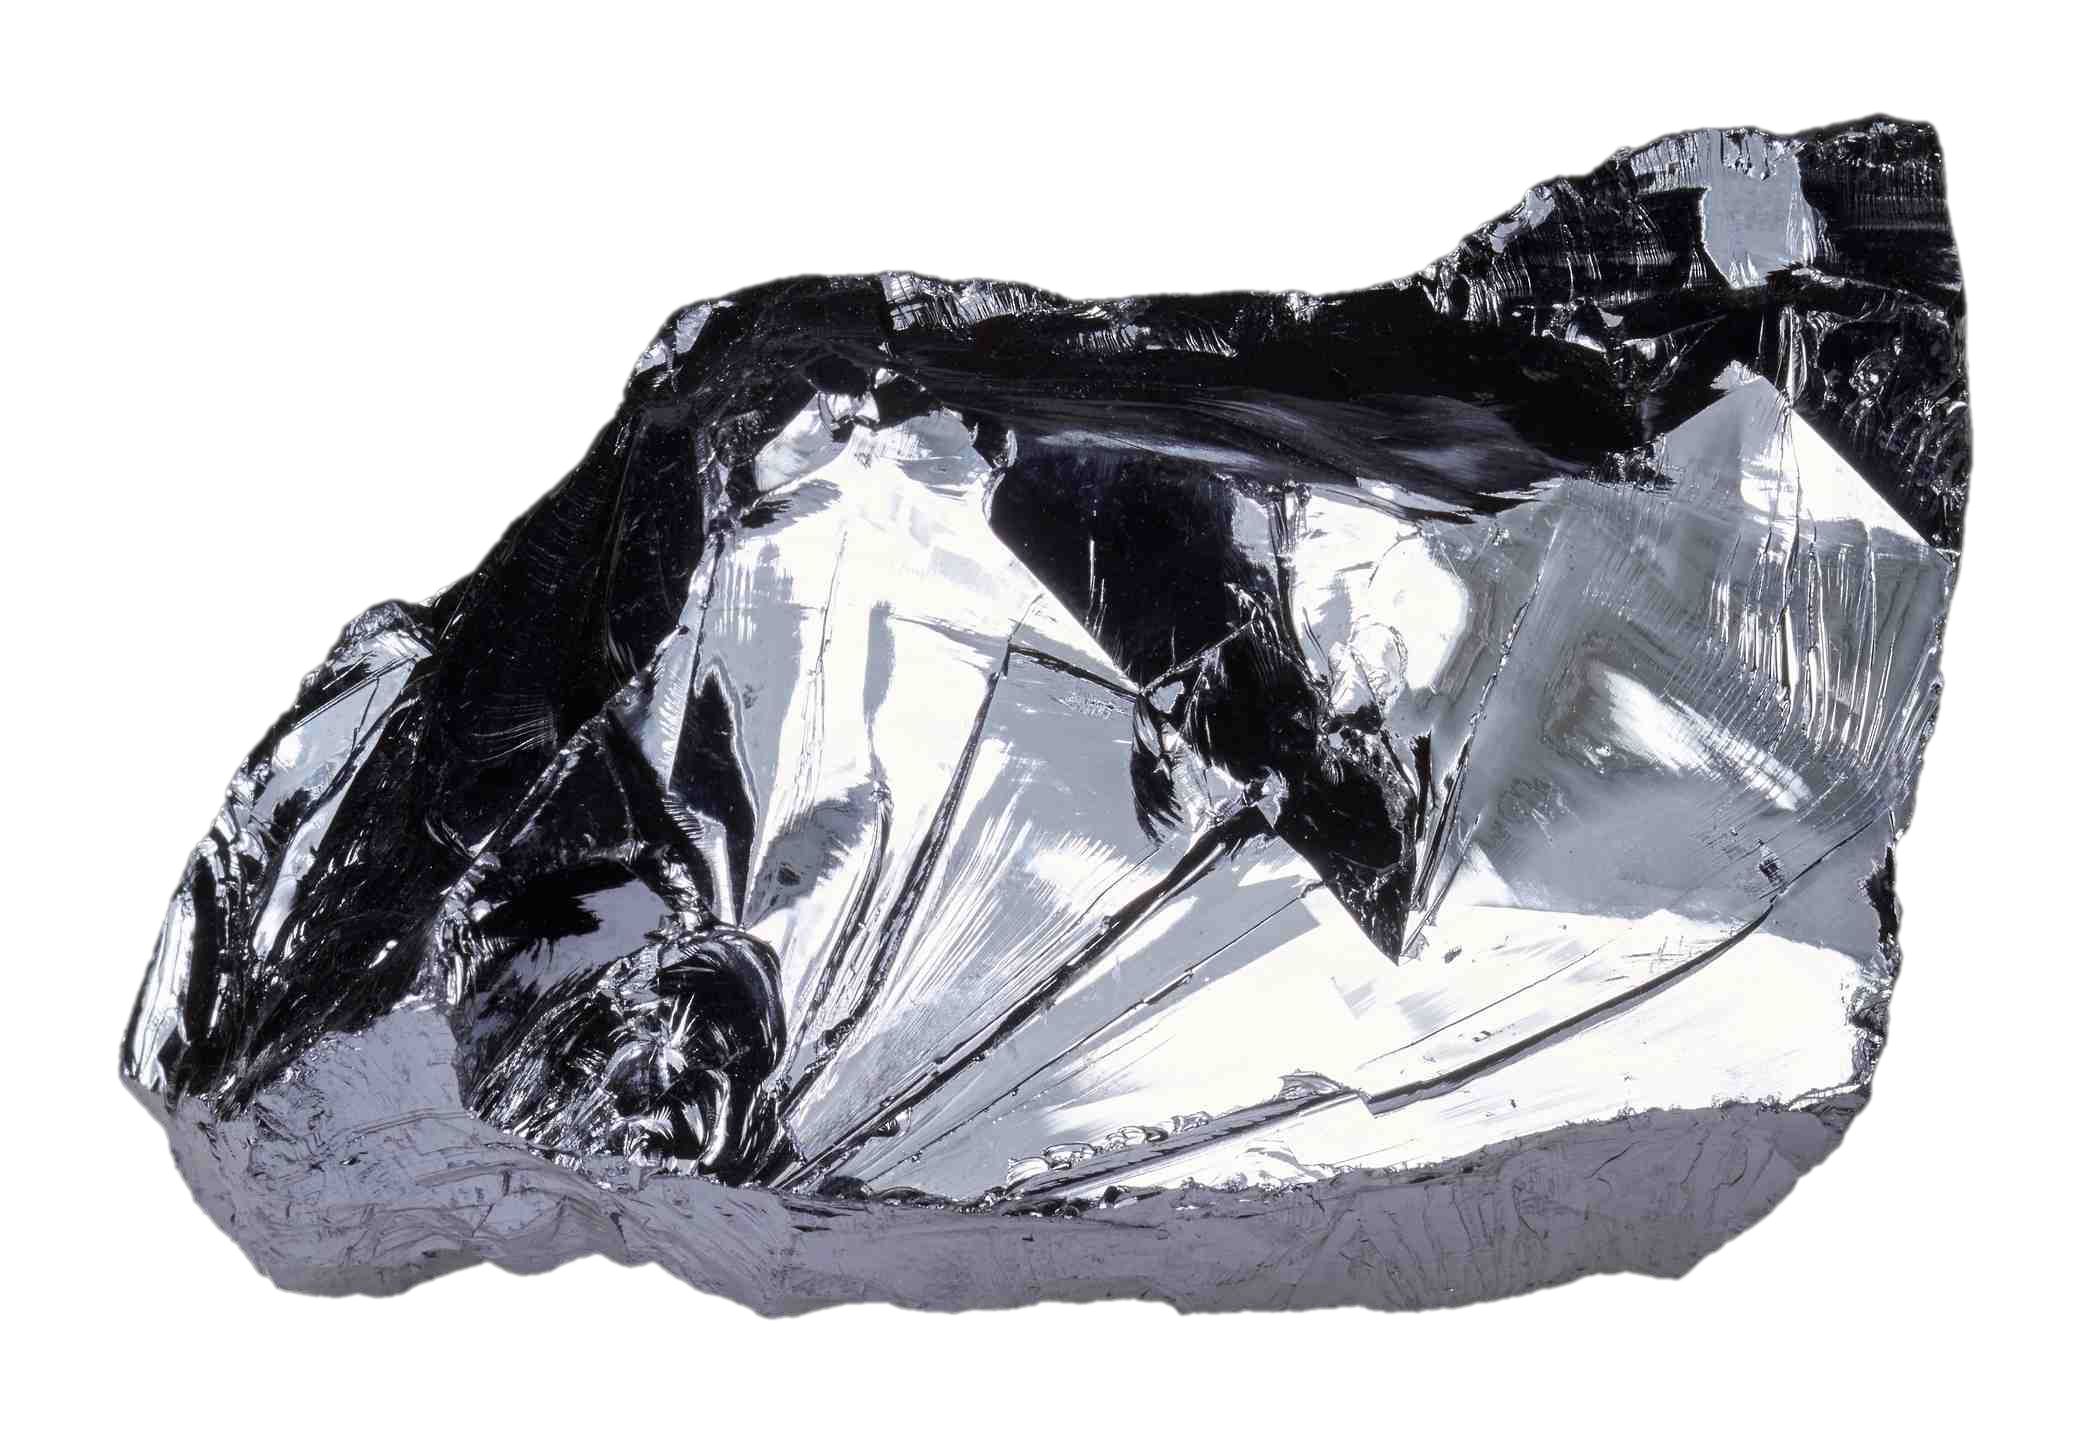
\includegraphics[width=.6\textwidth]{Sections/circuits/sicryst.jpg}
  \caption{An image of a silicon crystal \cite{gettyimages700832601}.}
  \label{fig:atom}
\end{figure}

\vspace{2em}
\begin{figure}[ht!]

  \centering
  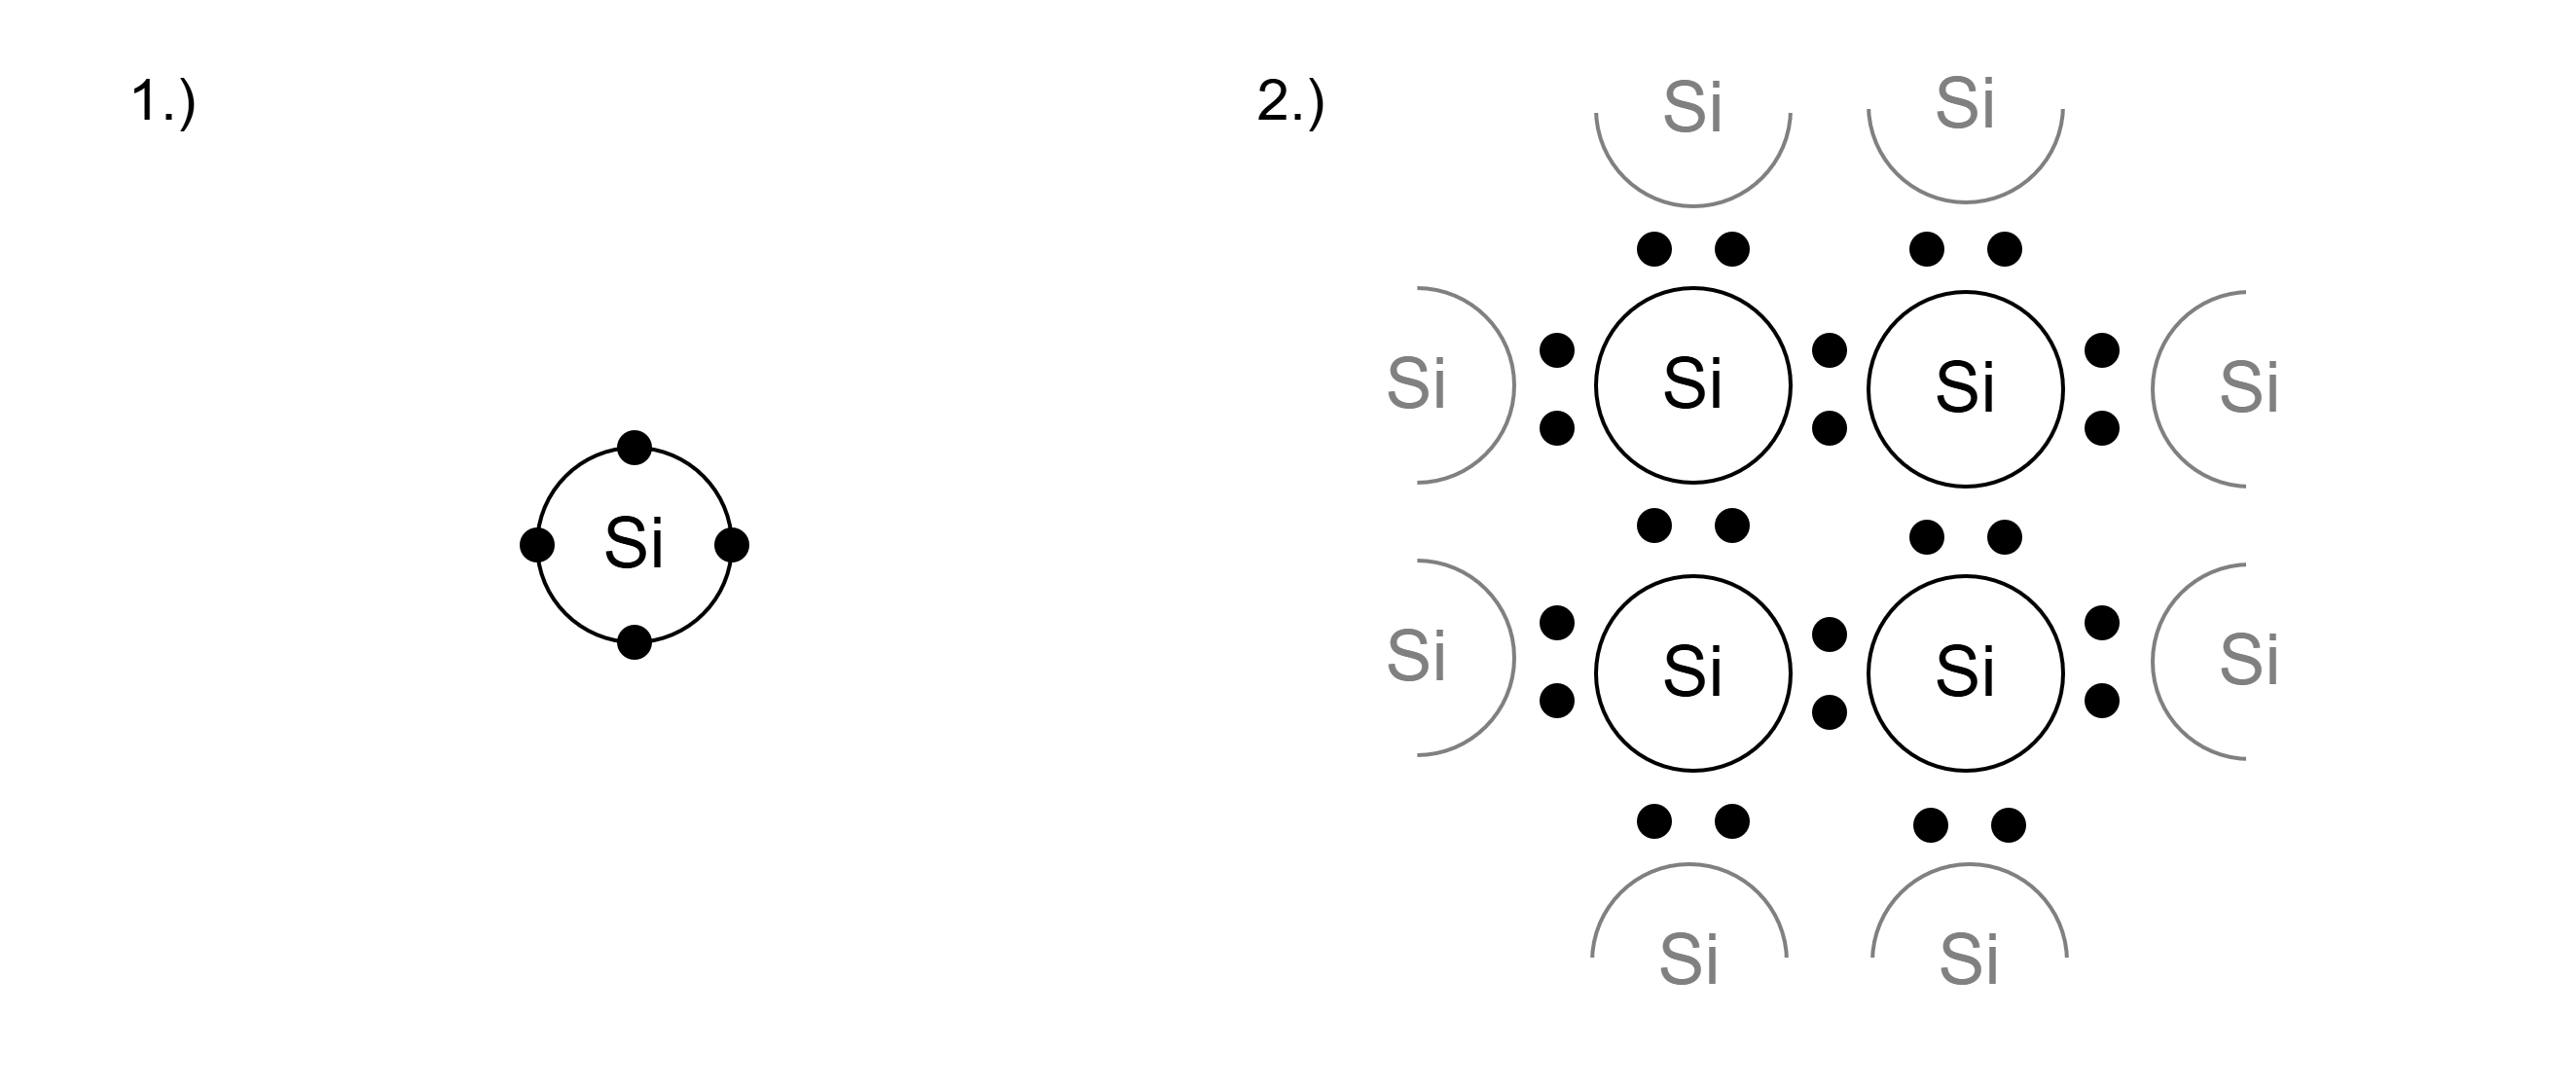
\includegraphics[width=\textwidth]{Sections/circuits/doping.png}
  \caption{(1) Shows a single silicon atom (Si) and its valence electrons (4 black dots).
  (2) Shows a flattened silicon lattice where neighboring Si atoms share their electrons to become stable.
  This creates an electron configuration of (2, 8, 8) for surrounded Si atoms.}
  \label{fig:doping}
\end{figure}
   
\newpage 

\noindent
\begin{figure}[ht!] 
  \centering
  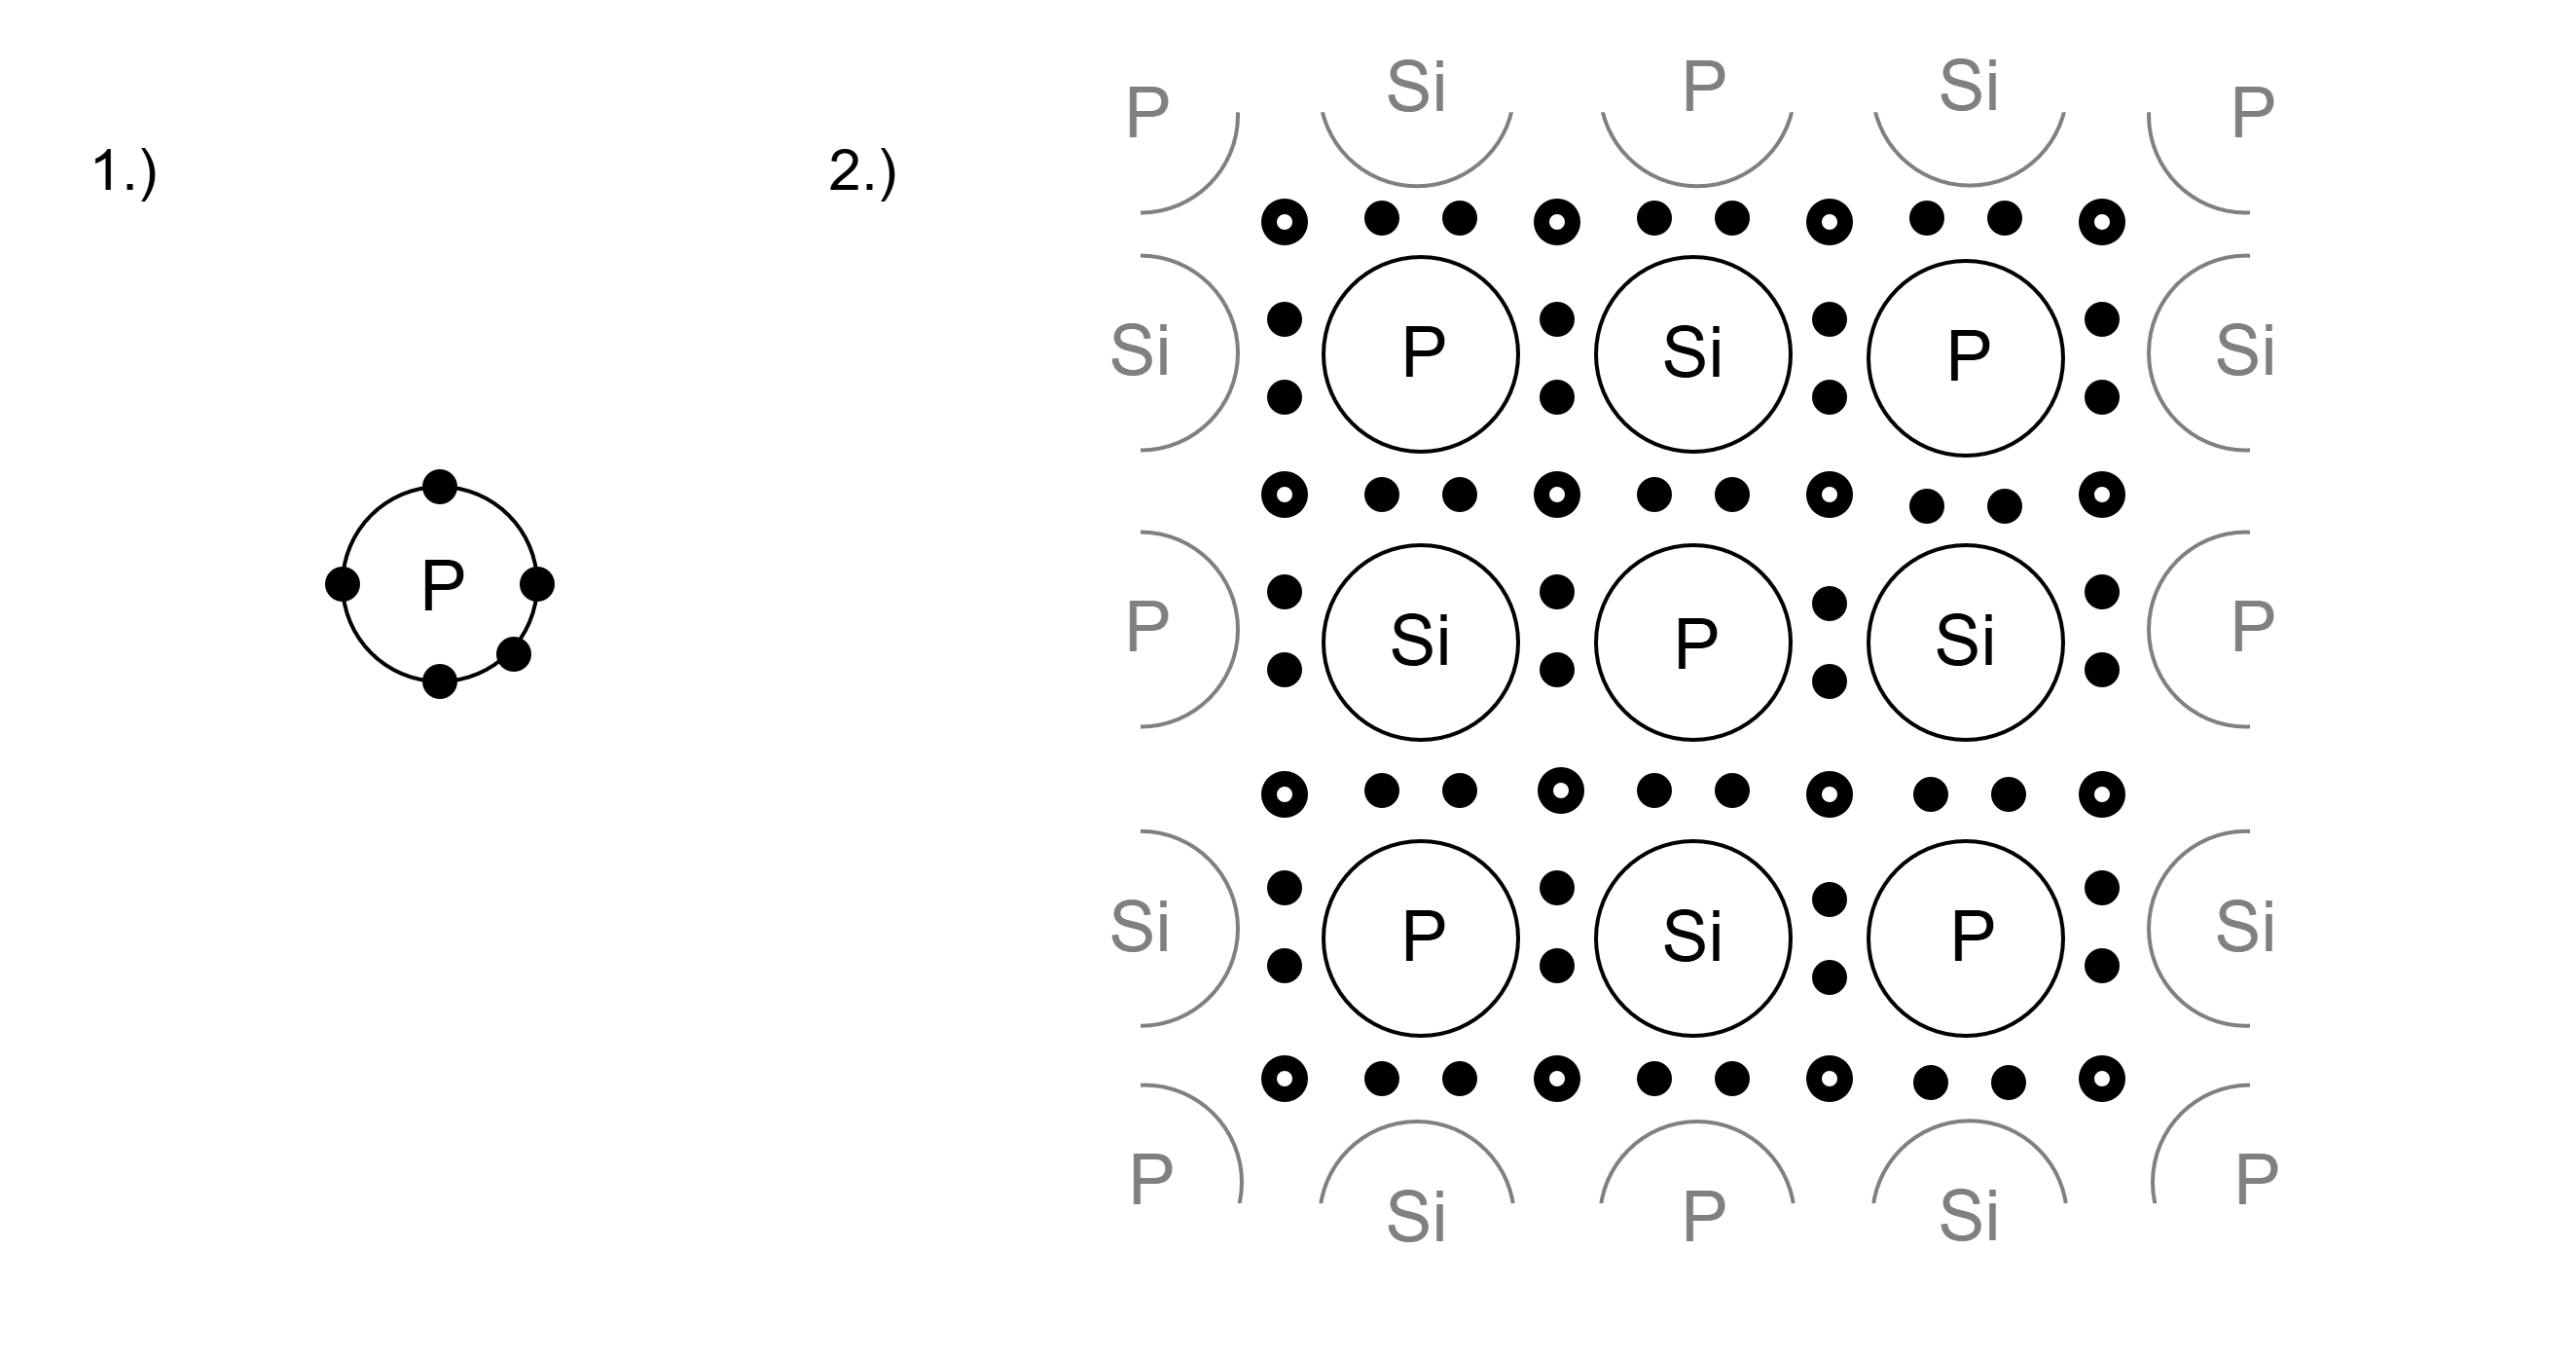
\includegraphics[width=\textwidth]{Sections/circuits/n-type.png}
  \caption{(1) Shows a single phosphorus atom (P) and its valence electrons (5 black dots).
  (2) A silicon lattice where phosphorus is doped, creating free electrons (thick dots with holes). }
  \label{fig:doping2}
\end{figure}

\vspace{-1em}
\begin{figure}[ht!]
  \centering
  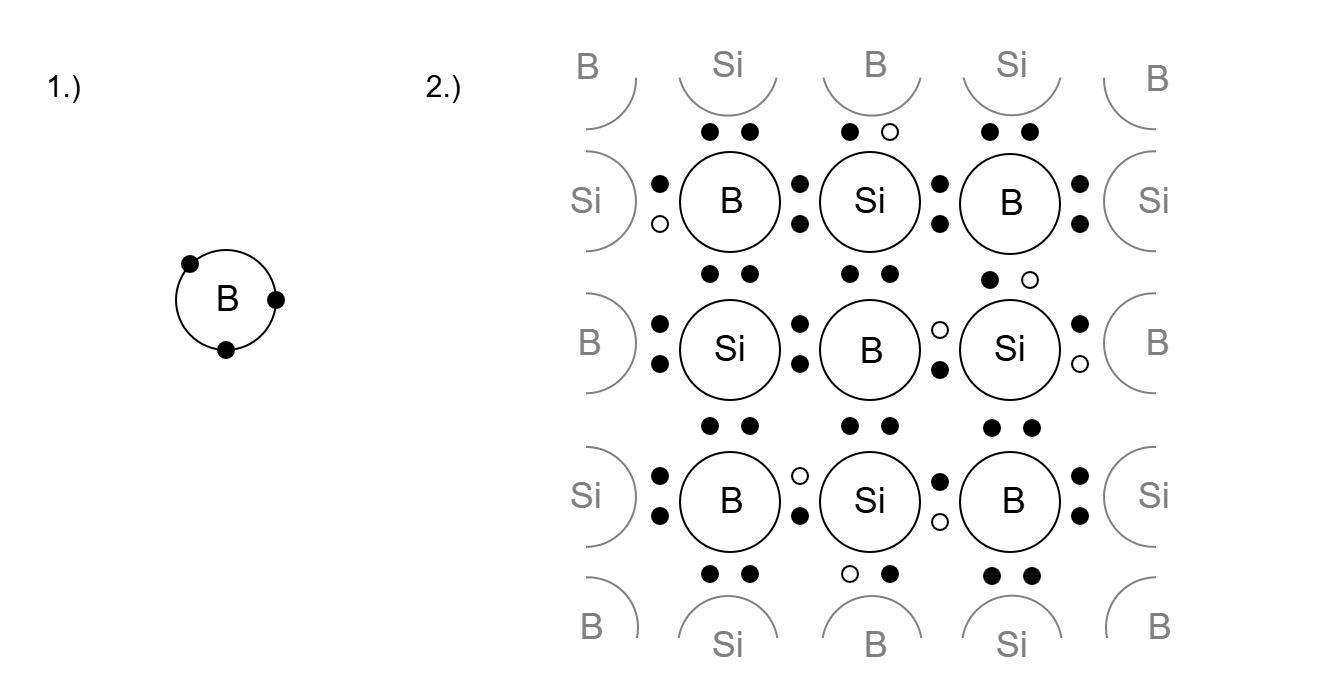
\includegraphics[width=\textwidth]{Sections/circuits/p-type.png}
  \caption{(1) Shows a single boron atom (B) and its valence electrons (3 black dots).
  (2) Shows a flattened silicon lattice where boron is doped, creating holes (halo dots). }
  \label{fig:doping3}
\end{figure}

\newpage 

\begin{Def}[N-type \& P-type Junctions]

    \label{def:n_p_junctions}

   When a N-type and P-type material are placed next to each other 
   creates a \textbf{PN-junction}. At this junction, we get a \textbf{depletion region},
   where N-type electrons and P-type holes cross; This leaves a 
   slightly positive region on the N-type side and a slightly negative region on the P-type side.
   This manifests an electric field, creating a barrier, preventing further flow across the junction \cite{engineermindset2024mosfet}.
\end{Def}

\vspace{-1.5em}
\noindent
\begin{figure}[ht!]
  \centering
  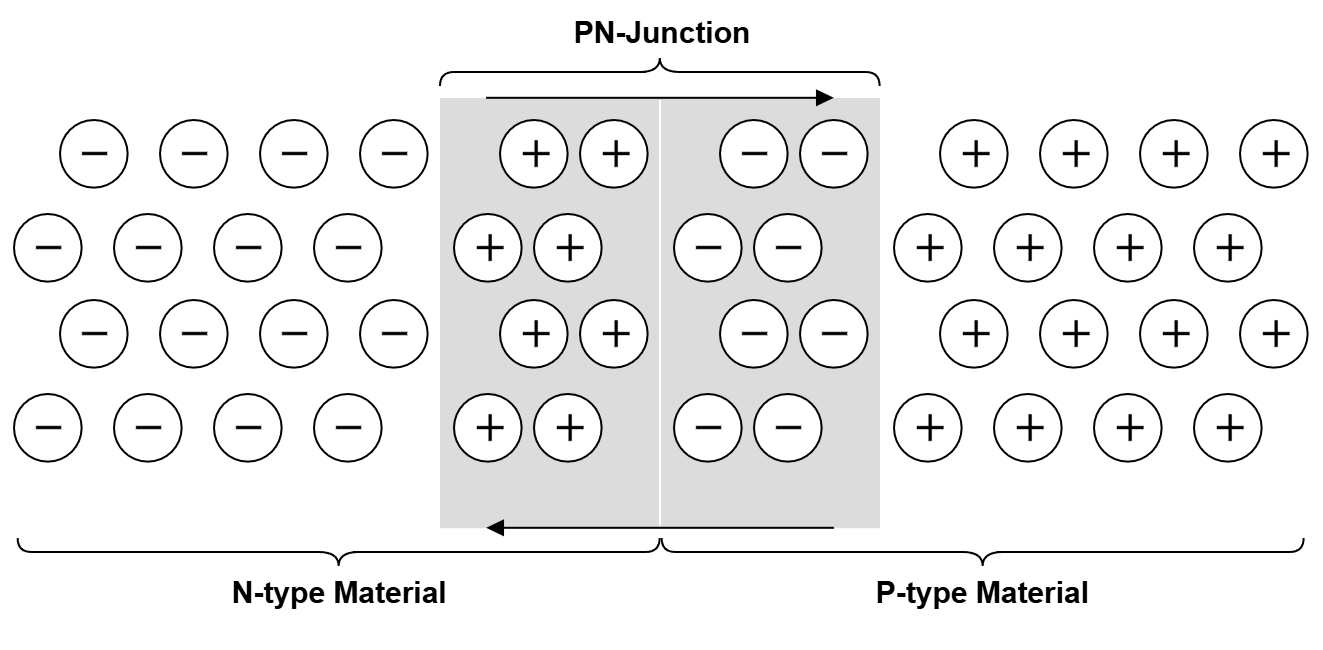
\includegraphics[width=\textwidth]{Sections/circuits/pn-junction.png}
  \caption{A PN-junction, where the depletion region is shown in gray.}
  \label{fig:pn-junction}
\end{figure}

\begin{Def}[MOSFET -- High-Level Overview]

    \label{def:mosfet_overview}
    \noindent
    A \textbf{MOSFET} (Metal-Oxide-Semiconductor Field-Effect Transistor) is a type of FET that uses its gate to control the flow of current.
    It consists of two default starting states:
    \begin{itemize}
      \item \textbf{Enhancement:} Normally \textbf{off} (i.e., no current flows), until such voltage is applied:
      \begin{itemize}
        \item \textbf{N-Channel Enhancement:} A positive voltage.
        \item \textbf{P-Channel Enhancement:} A negative voltage.
      \end{itemize}
      \item \textbf{Depletion:} Normally \textbf{on} (i.e., current flows), until such voltage is applied:
      \begin{itemize}
        \item \textbf{N-Channel Depletion:} A negative voltage.
        \item \textbf{P-Channel Depletion:} A positive voltage.
        \end{itemize}
    \end{itemize}
  \end{Def}

\newpage 

\begin{Def}[MOSFET -- Anatomy of N-Channel]

    \label{def:mosfet}

    A MOSFET \textbf{N-Channel Enhancement} is constructed as follows:
    \begin{itemize}
      \item \textbf{Substrate:} A base-layer of P-type material from which all parts will build upon.
      \item \textbf{Source \& Drain:} Two motes are dug at either ends of the substrate and filled with N-type material;
      One for our \textbf{source} and the other for our \textbf{drain}. Two metal contacts are placed on these motes (our terminals);
      A body of metal is connected to the bottom of the substrate (\textbf{base/body terminal}), which connects to the source terminal.
      \item \textbf{Gate:} A metal contact pad is placed between the motes on top of the SiO$_2$ layer, forming the \textbf{gate terminal}.
      A layer of silicon dioxide (SiO$_2$) is sandwiched between the gate and the substrate.
      Since SiO$_2$ is a superb insulator, it prevents the gate terminal from touching/interacting with the substrate.
      \item \textbf{Channeling:} SiO$_2$ is a \textbf{dielectric} material, meaning that when a charge is applied to one side, the opposite charge builds on the other side,
      creating an electric field. When a positive charge is applied, it attracts negative electrons from the other side, creating a \textbf{channel} (i.e., bridge)
      between the two motes (source to drain), allowing current.
    \end{itemize}
    
    \noindent
    The \textbf{M}etal from gates, the \textbf{O}xide from the SiO$_2$ layer, the \textbf{S}emiconductor from the substrate and motes, and 
    the \textbf{FET} from the field-effect, gives us the name \textbf{MOSFET}.

    \noindent
    \rule{\textwidth}{0.4pt}\\
    \noindent
    For \textbf{N-Channel Depletion}, A \emph{thin} N-type substrate-channel is already present, bridging the two motes (source and drain) together.
    Once a negative charge is applied to the gate, positive holes are attracted, weakening the channel; This effectively stops the flow of current.
\end{Def}

\vspace{-1em}
\begin{figure}[ht!]
  \centering
  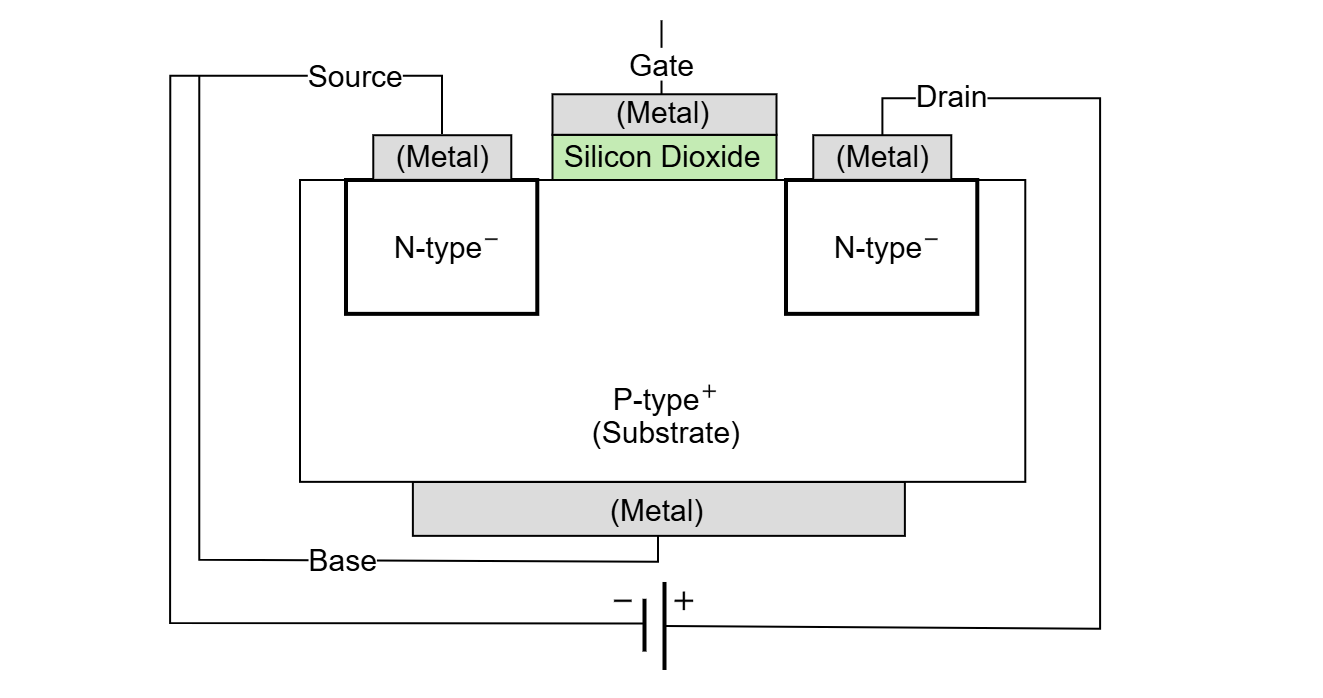
\includegraphics[width=.91\textwidth]{Sections/circuits/mosfet.png}
  \caption{N-Channel Enhancement (off). Negative battery side to source, positive to drain.}
  \label{fig:mosfet}
\end{figure}

\newpage

\begin{theo}[Flow of Electrons]

  \label{theo:flow_of_electrons}

  Recall that a body of electrons that are negatively charged (low potential), have a surplus of electrons.
  A positive charge (high potential) reflects a deficit of electrons. Therefore, when given the chance
  (alike water), electrons will flow to fill the void.
\end{theo}

\begin{Tip} An empty stomach has a high potential for food, while a full stomach has a low potential,
  as there's not much more room left to stuff food into.
\end{Tip}

\begin{Def}[MOSFET -- N-Channel Battery Configuration]

    \label{def:mosfet_gate_interaction}

    One battery is used to power the MOSFET, and another to control the gate.
    The source connects to the negative, and the drain to the positive side of the battery.
    
    The gate is connected to a second battery, which can be either positive or negative, depending on the MOSFET type.
    The \textbf{other} end of this battery is connected to the source terminal.
\end{Def}

\begin{figure}[ht!]
  \centering
  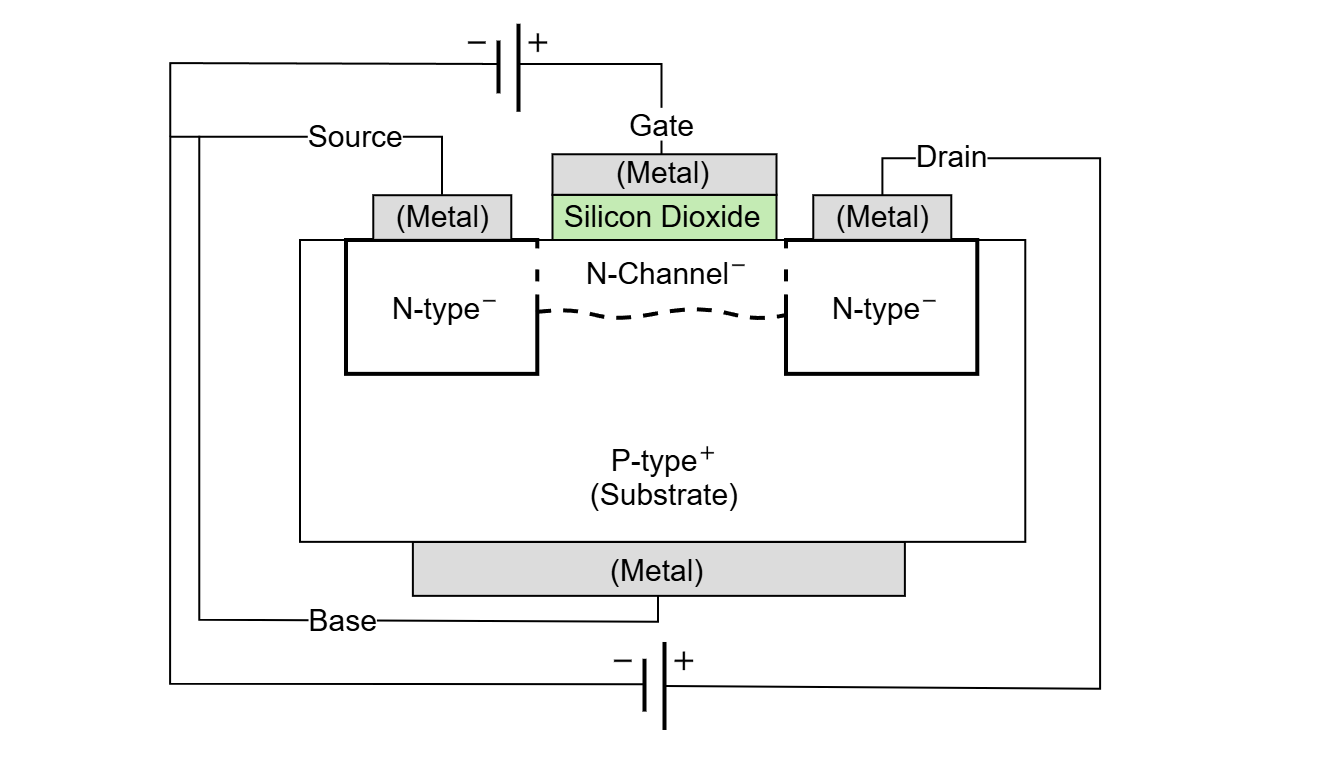
\includegraphics[width=.91\textwidth]{Sections/circuits/mosfet-on.png}
  \caption{N-Channel Enhancement (on). Negative battery side to gate, positive to source.
  Positive charge given to the gate attracts negative electrons on the other side of the 
  SiO$_2$ layer, creating a channel between the source and drain.}
  \label{fig:mosfet-on}
\end{figure}


% \begin{Tip} The same goes with heat, there technically is no such thing as the
%   ``cold'', it is just the lack of heat. At a high-level, heat is how fast atoms are jittering around.

%   Though for different reasons, heat rushes into the cold as it's ``jittery'' while the cold is ``still''.
%   Analogously, its relatively easier to run across a forest of trees than a field of dancing people; The chance
%   of bumping into someone knocking you off course than a tree is much higher.
% \end{Tip}

\newpage 

\begin{figure}[ht!]
  \centering
  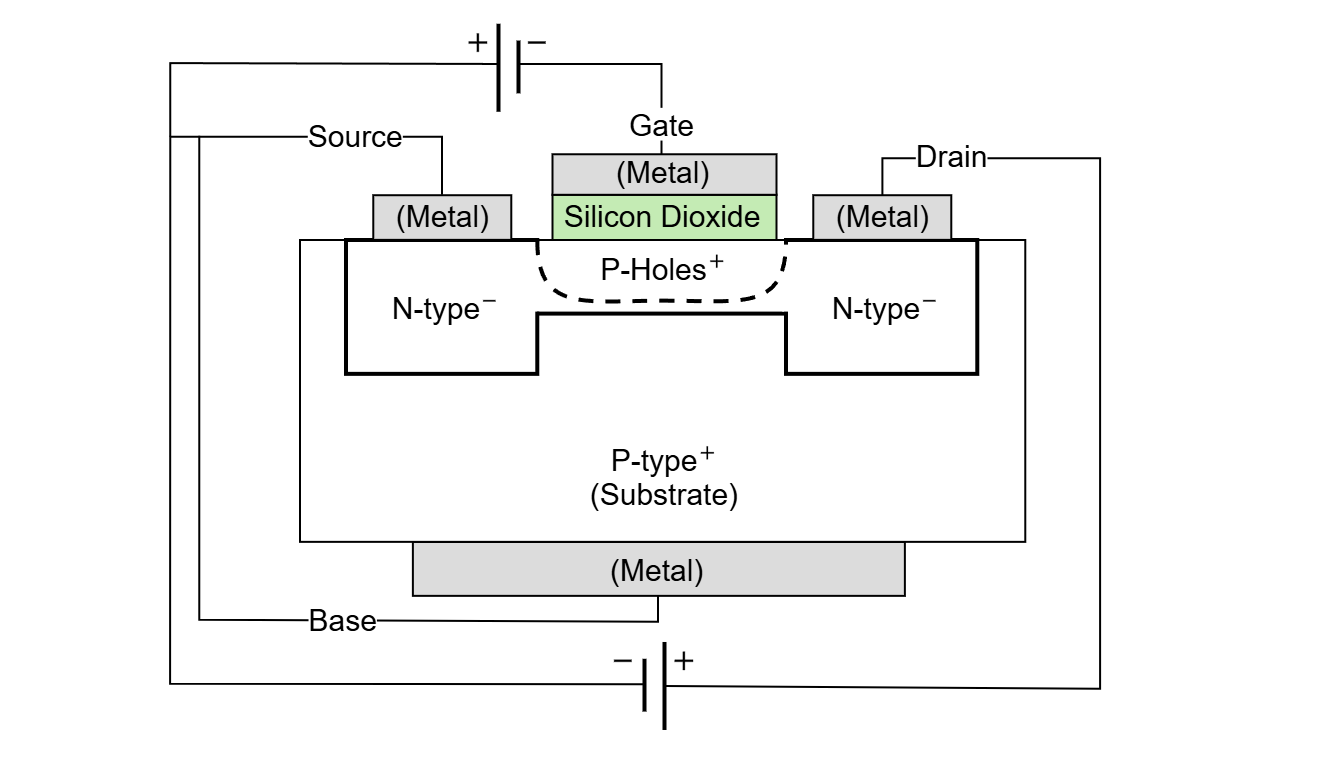
\includegraphics[width=.91\textwidth]{Sections/circuits/mosfet-depletion.png}
  \caption{N-Channel Depletion (on). Negative charge to gate, creates holes into the channel.}
  \label{fig:mosfet-depletion}
\end{figure}

\vspace{-1em}
\begin{Def}[MOSFET -- Anatomy of P-Channel]

    \label{def:mosfet_p_channel}

    The P-Channel variation follows the same logic as the N-Channel Definition (\ref{def:mosfet});
    Instead, we swap N-type for P-type materials, and vice versa. Then apply negative for Enhancement
    and positive for Depletion on the gate to open or close the channel respectively (\ref{def:mosfet_overview}).
    \textbf{In particular}, source now connects to a high potential and drain to a low potential.

\end{Def}

\vspace{-1em}
\begin{figure}[ht!]
  \centering
    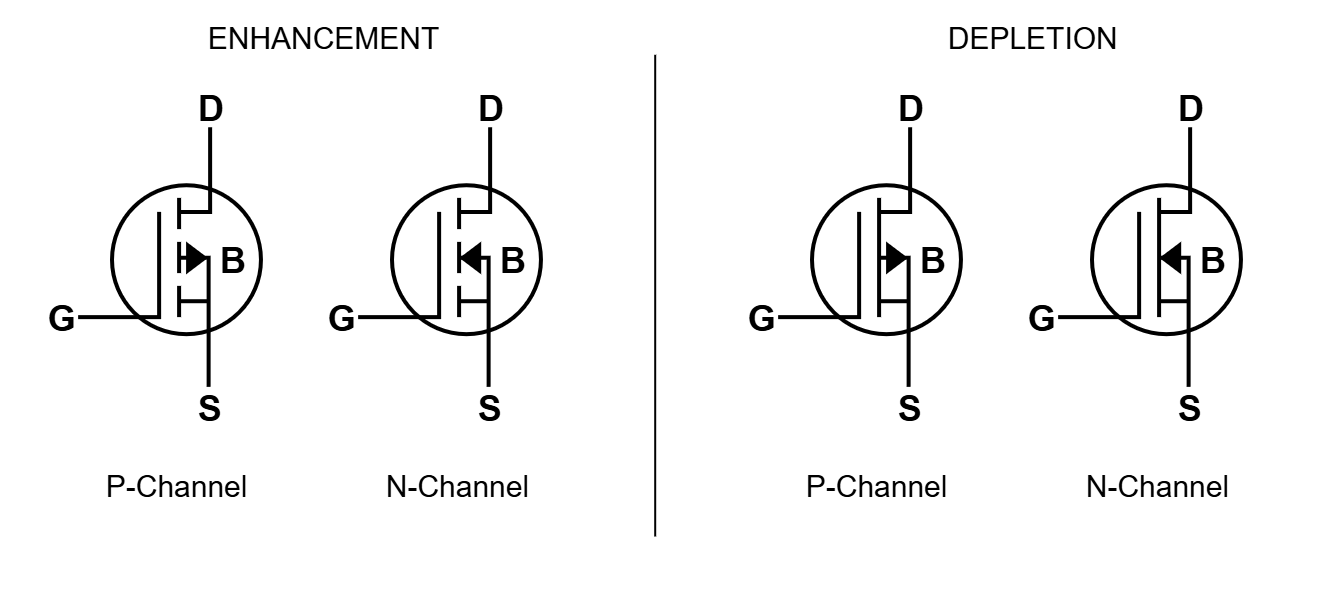
\includegraphics[width=.9\textwidth]{Sections/circuits/mosfet-symbol.png}
  \caption{MOSFET symbols, \textbf{G} (gate), \textbf{S} (source), \textbf{D} (drain), and \textbf{B} (body) terminals.}
  \label{fig:mosfet-symbol}
\end{figure}

\newpage 

\subsection{Logic Gates \& Functional Completeness}

\noindent
This section will cover how we take MOSFETs and use them to build logic gates.

\begin{Def}[Gate-Source Voltage $V_{GS}$]

  \label{def:gate_source_voltage}

  Recall Definition (\ref{def:mosfet_gate_interaction}), the gate battery's opposite end is connected to the source terminal.
  This serves as a zero-volt reference for the gate terminal.
  The difference in potential between the gate and source terminals is called the \textbf{gate-source voltage} ($V_{GS}$):
  \[
    V_{GS} = V_{G} - V_{S},
  \]
  
  \noindent
  Once $V_{GS}$ exceeds the threshold voltage $V_{TN}$ (for N-channel) or is below the threshold voltage $V_{TP}$ (for P-channel), the MOSFET turns on, allowing current to flow from source to drain.
\end{Def}

\begin{Tip} Notice that source takes from gate, i.e., for N-channel, the gate must overcome the source's 
  negative charge. Hence we must exceed a threshold voltage to turn on the MOSFET.
  For P-channel, the same logic applies, but in reverse, as the components are implemented in a complementary manner.
\end{Tip}

\begin{Def}[Pull-Up \& Pull-Down Switches]

  \label{def:pull_up_down_switches}

  Let $V_{DD}$ be the positive supply (“logical 1”) and ground (0 V) be “logical 0.”  A CMOS logic gate uses:
  \begin{itemize}
    \item \textbf{Pull-Down Switch} (Off: 0, On: 1): N-channel enhancement. If $V_{GS} > V_{TN}$, source connects to drain, producing a logical 1.
    \item \textbf{Pull-Up Switch} (Off: 1, On: 0): P-channel enhancement. If $V_{GS} < V_{TP}$, source connects to $V_{DD}$, producing a logical 1.
  \end{itemize}
\end{Def}
\begin{Tip} Think of pull-down as ``pulling down to the ground'' to allow electrons to escape.

  Additionally, the ``DD'' in $V_{DD}$ does not stand for anything; it was made not to be confused with 
  $V_D$, the voltage at the drain terminal. Though, unimaginative, it is simply convention.
\end{Tip}
\newpage 

\begin{Def}[CMOS Logic Gate]

  \label{def:cmos_logic_gate}

  A \textbf{CMOS logic gate} is a circuit that uses \textbf{C}omplementary \textbf{MOS}FETs to perform logical operations. It consists of:
  \begin{itemize}
    \item \textbf{Pull-Down Network (PDN):} N-channel MOSFETs (NFET) connected to ground.
    \item \textbf{Pull-Up Network (PUN):} P-channel MOSFETs (PFET) connected to $V_{DD}$.
  \end{itemize}
  
  \noindent
  The output is high when the PUN is active and the PDN is inactive, and vice versa.
\end{Def}

\vspace{-1em}
\begin{figure}[ht!]
  \centering
  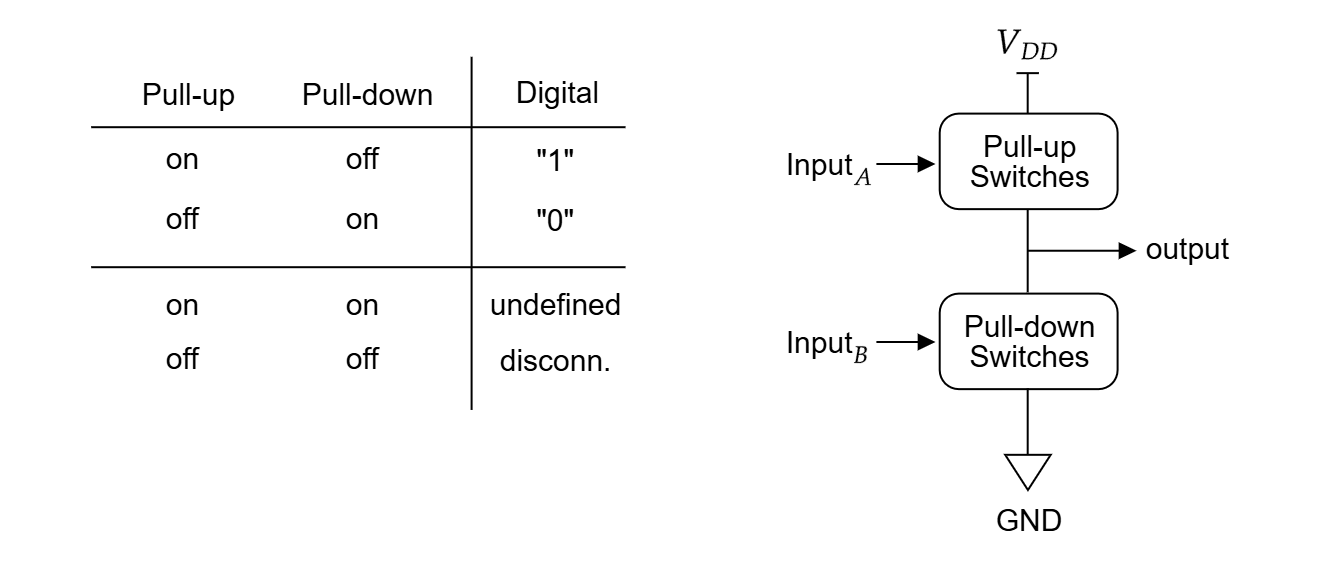
\includegraphics[width=\textwidth]{Sections/circuits/pun_pdn.png}
  \caption{Simple CMOS logic gate, where \textbf{GND} stands for ground, \textbf{$V_{DD}$} for positive supply.
  \textbf{Note:} That even if the circuit is disconnected, the output may still \emph{``remember''} its last state for some 
  time until the charge dissipates.}
  \label{fig:cmos-logic-gate}
\end{figure}

\begin{Def}[Simplified NFET \& PFET Symbols]

  \noindent
  Below are input gates $A$ and $B$, with two other terminals $T_1$ and $T_2$, simplifying Figure(\ref{fig:cmos-logic-gate}):

  \begin{center}
    
    
\includegraphics[width=\textwidth]{Sections/circuits/np_simp.png}
  \end{center}
  
  \noindent
  (1) NFET, $T_1$ output, and $T_2$ ground; (2) PFET, $T_1$ is $V_{DD}$ (typically 1V), and $T_2$ output \cite{youtube:1rZyGL1K5QI}.

\end{Def}

\newpage

\noindent
\begin{Def}[Open \& Closed Circuits -- NFET \& PFET Logic]

  \label{def:open_closed_circuits}

  A \textbf{closed circuit} is a complete path for current to flow, while an \textbf{open circuit} is an incomplete path:

  \begin{center}
  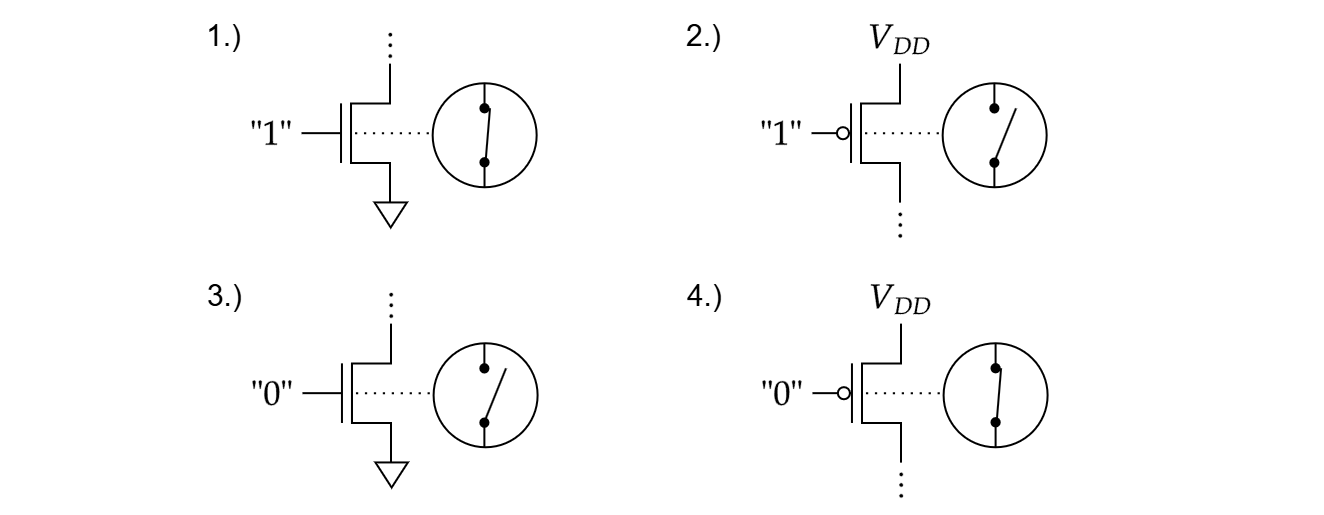
\includegraphics[width=\textwidth]{Sections/circuits/open_closed.png}
  \end{center}

  \noindent
  (1) An NFET is closed when given a digital 1 (high voltage), while (2) a PFET, is open;\\
  (3) NFET, open when given 0 (low voltage), while (4) a PFET is closed.
\end{Def}

\begin{Def}[MOSFET Logic Gate -- Not]

  \label{def:mosfet_logic_gate_not}

  Below shows a logic gate, NOT, using MOSFETs (NFET and PFET):

  \begin{center}
  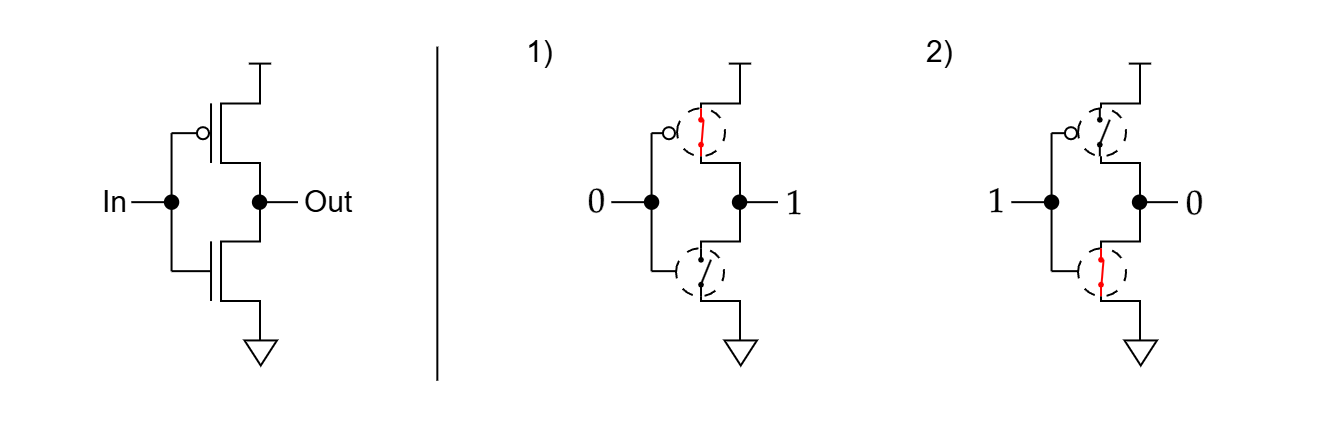
\includegraphics[width=\textwidth]{Sections/circuits/not.png}
  \end{center}

  \noindent
  Both the NFET and PFET share the same input. The top line represents $V_{DD}$ (positive supply), while the bottom line is ground (triangle).
  (1) input low, NFET is open, PFET is closed, output is high from $V_{DD}$; (2) input high, NFET is closed, PFET is open, output is low from ground.
  \textbf{Important:} A black dot connecting two or more lines represents a connection.
\end{Def}

\newpage 

\begin{Def}[Functional Completeness]

  \label{def:functional_completeness}

 it can be used to express all possible Boolean functions.
    For example, the set of operators $\{\text{AND, OR, NOT}\}$ is functionally complete.
    However, we can do better. The NAND gate (and NOR gate) by itself is functionally complete.
\end{Def}

\begin{Example}[Functionally Complete Sets of Operators]

    \begin{enumerate}
  \item $\{\mathrm{NAND}\}$ alone
    \begin{align*}
      \neg A &= A \operatorname{NAND} A,\\
      A\land B &= \neg\bigl(A \operatorname{NAND} B\bigr)
                = \bigl(A \operatorname{NAND} B\bigr)\operatorname{NAND}\ \bigl(A \operatorname{NAND} B\bigr),\\
      A\lor B  &= (A \operatorname{NAND} A)\operatorname{NAND}\ (B \operatorname{NAND} B).
    \end{align*}

  \item $\{\mathrm{NOR}\}$ alone
    \begin{align*}
      \neg A &= A \operatorname{NOR} A,\\
      A\lor B  &= \neg\bigl(A \operatorname{NOR} B\bigr)
                = \bigl(A \operatorname{NOR} B\bigr)\operatorname{NOR}\ \bigl(A \operatorname{NOR} B\bigr),\\
      A\land B &= (A \operatorname{NOR} A)\operatorname{NOR}\ (B \operatorname{NOR} B).
    \end{align*}

    \item $\{\land,\neg\}$ alone
    \begin{align*}
      \neg A   &= \neg A,\\
      A\land B &= A\land B,\\
      A\lor B  &= \neg\bigl(\neg A \land \neg B\bigr).
    \end{align*}

  \item $\{\lor,\neg\}$ alone
    \begin{align*}
      \neg A   &= \neg A,\\
      A\lor B  &= A\lor B,\\
      A\land B &= \neg\bigl(\neg A \lor \neg B\bigr).
    \end{align*}

  \item $\{\to,\neg\}$ alone
    \begin{align*}
      \neg A   &= \neg A,\\
      A\lor B  &= \neg A \to B,\\
      A\land B &= \neg\bigl(A \to \neg B\bigr).
    \end{align*}
\end{enumerate}

\noindent
Recall, $A \to B$ is logically equivalent to $\neg A \lor B$. 
\end{Example}

\newpage 

\noindent
Let's brainstorm possibilities for an AND and NAND, and elaborate on Defintition (\ref{def:cmos_logic_gate}):
\begin{theo}[Balancing Series \& Parallel Connections]

  \label{theo:balancing_series_parallel}

    \noindent
    It's important in a CMOS circuit that the PUN and PDN are in fact complements of each other. Below
    illustrates two types of connections:

    \begin{center}
      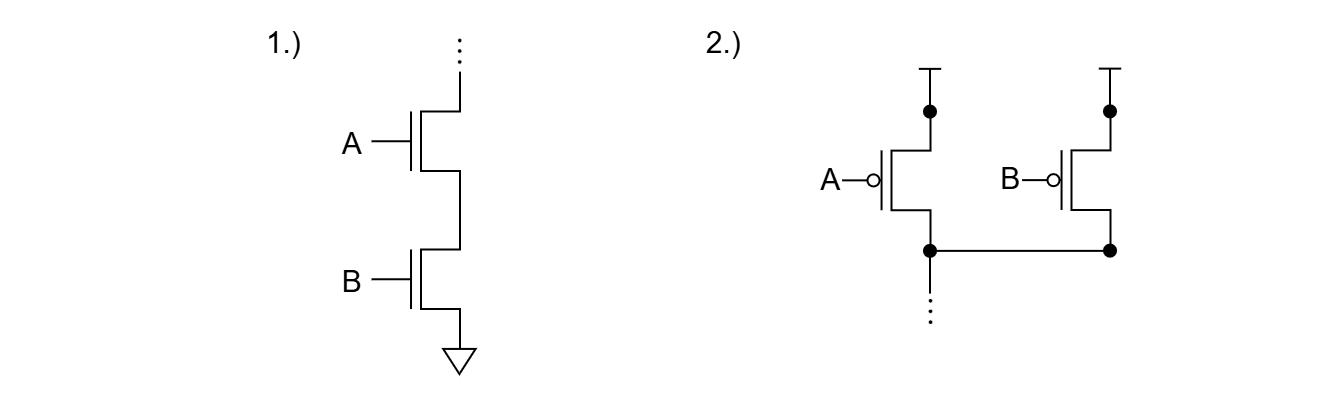
\includegraphics[width=\textwidth]{Sections/circuits/np_comp.png}
    \end{center}

    \noindent
    (1) Shows a NFET \textbf{series} connection (i.e., sequentially connected). Theoretically in isolation, this represents
    an AND gate ($A \cdot B$), meaning both $A$ and $B$ must be high to close the circuit. 
    
    (2) Shows a PFET in \textbf{parallel} connection (i.e., side-by-side connected). As per complementarity, this represents the NAND gate
    ($\overline{A} + \overline{B} = \overline{A \cdot B}$), by De Morgan's Law; Either $A$ or $B$ must be low to close the circuit.\\
    \rule{\textwidth}{0.4pt}\\
    \noindent
    Hence to \textbf{balance}, between the PUN and PDN, we must ensure that:
    \begin{itemize}
        \item each NFET series requires a PFET parallel.
        \item each PFET series requires a NFET parallel.
    \end{itemize}

    \noindent
    This keeps our networks complementary, ensuring that \underline{when one is closed, the other is open}.
\end{theo}

\begin{Tip} Think about how to create this before moving to the next page.
  understand that the placement of the output determines the logic of the circuit. 
  Since PUNs default to high, think about how that might affect the output.

  In CMOS, there must be both a PUN and PDN, think about how to balance the (2), from the above Theorem (\ref{theo:balancing_series_parallel}), to create a NAND gate.
\end{Tip}



\newpage
\begin{theo}[CMOS Logic Gate -- NAND]

  \label{def:mosfet_logic_gate_nand}

  \noindent
  Combining both networks in Theorem (\ref{theo:balancing_series_parallel}) yields a NAND gate in the following configuration:

  \begin{center}
    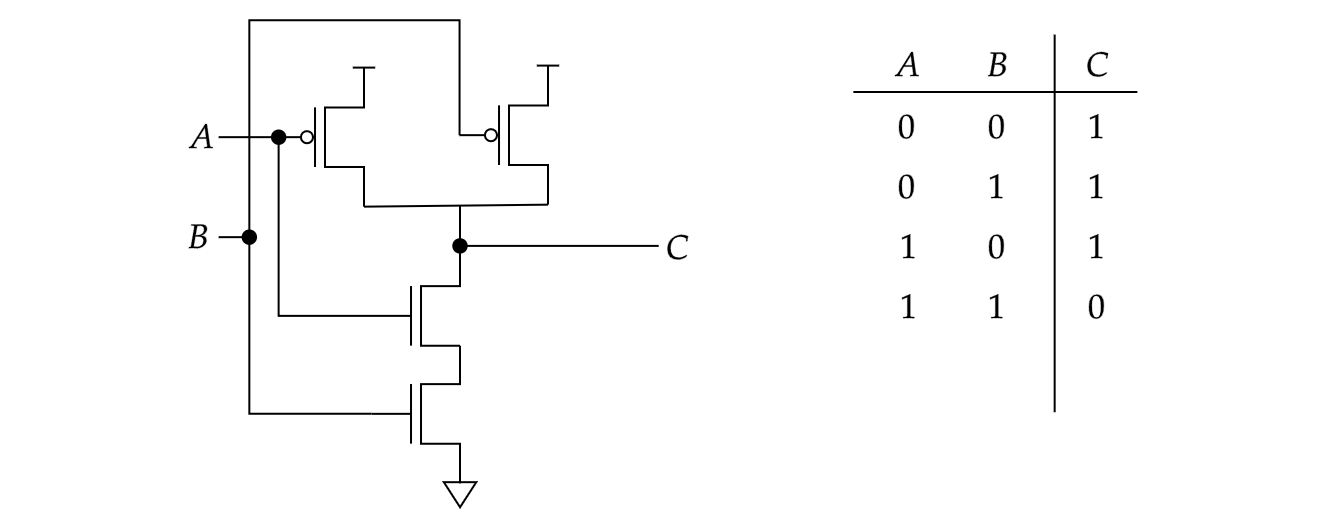
\includegraphics[width=\textwidth]{Sections/circuits/nand.png}
  \end{center}
\end{theo}

\vspace{2em}
\begin{figure}[ht!]
  \centering
  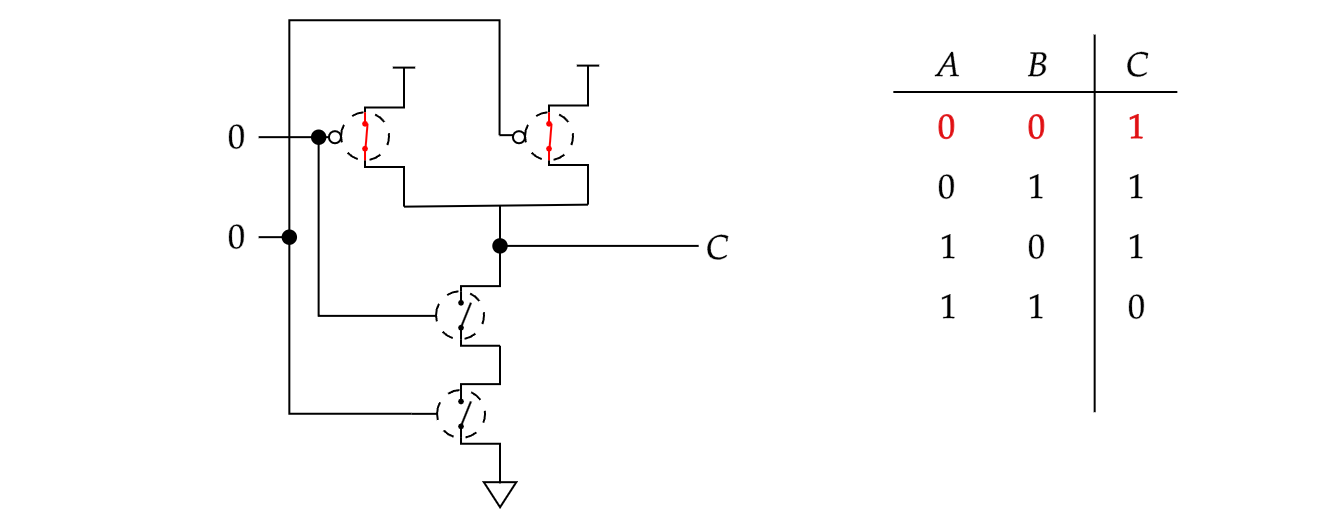
\includegraphics[width=\textwidth]{Sections/circuits/nand_1.png}
  \caption{Both inputs are (0,0), PUN closed, PDN open, hence the output is high (1).}
  \label{fig:nand-1}
\end{figure}

\begin{figure}[ht!]
  \centering
  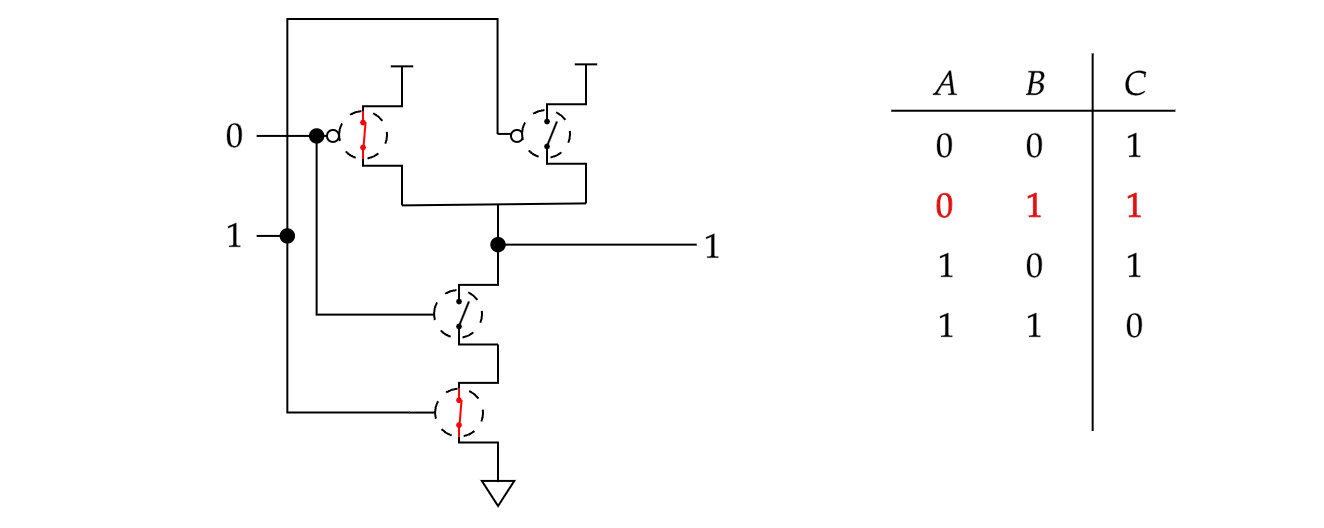
\includegraphics[width=\textwidth]{Sections/circuits/nand_2.png}
  \caption{Both inputs are (0,1), PUN half-closed reaching the output, PDN half-closed, but can't reach the output; Hence the output is high (1).}
  \label{fig:nand-2}
\end{figure}

\newpage 

\noindent
(Taking a break from writing. I intended to write all the way to show 
how with the PUN and PDN configurations achieve binary addition, subtraction, multiplication, and division.
But I think this is enough for now. I will come back to it later.)